\fancyhead[R]{Leonie Boland}
\subsection{Deep-Q Learning Agent} \label{sec:deepqtraining}

\subsubsection{Training Environment Progression}

We always conducted a similar training routine, namely starting off with a small field with height and width of 7 containing coins on every tile, so 21 coins in total. This game environment is called coin heaven in the following. Starting the training with this scenario gave us the opportunity to already evaluate if there are flaws in the implementation or how fast the network converges with the chosen hyperparameters. This is evaluated in more detail in section \ref{sec:deepqexperiments}. Then we scaled the field up to 11 $\times$ 11 and increased the difficulty by including crates. In this environment, called loot crate, we included 20 coins and used a crate density of 40\%. Finally the agent was trained with all settings as in the target field, that is a 17 $\times$ 17 field, 9 coins and a crate density of 0.75. The last step was to add opponents to this classic environment to train in the exact same environment our agent will be tested in. Simultaneously to raising size and difficulties we also increased the steps per round from 60 to 120 to 200, as the agent does not need 200 steps to collect all coins in a field as small as 7 $\times$ 7.

\subsubsection{Self-Play Strategy}

After the agent was trained without opponents to learn the basic skills like dropping a bomb to destroy crates, escaping that bomb and collecting coins, the agent needed to find out how to compete against opponents. This is where self-play comes into action. Utilizing the self-play strategy means that the model is trained while competing against itself. The advantage of this training strategy is, that the opponent has a similar level. This is desirable as a too weak opponent would not force the model to find a way to play a game more efficiently. Actually, the worst case scenario would be, that the agent learns nothing new in comparison to running the game without opponents. However, a too strong opponent would take the opportunity to learn something away from our agent, as the other opponent would collect the coins faster or kill our agent easily. Hence, we trained our agent against itself and our not training agent reloaded the model that is currently trained after every 500 rounds. As the agent improves over time, it faces progressively more challenging opponents, leading to continuous improvement and skill development. \cite{selfplay} Sadly, we only explored this strategy after handing in our best running agent at the time of the deadline. We have no data to proof that the self-play trained agent excels the previous agent but our hypothesis is, that it does.

\subsubsection{Auxiliary Rewards} \label{sec:rewards}

The basic concept of reinforcement learning is, to give the agent rewards depending on the action taken in a game state that leads to a new game state. In the case of Bomberman the agent could learn the essentials to play the game by getting a reward respectively a penalty for the standard events that can occur. The standard events we chose to reward are "coin collected", "invalid action", "crate destroyed", "got killed",  "killed opponent", "killed self", "survived round" and "waited". In theory the model should be able to learn how to play the game well just by receiving appropriate positive rewards for collecting a coin, destroying crates, killing opponent and surviving one game round, and negative rewards for taking an invalid action, getting killed by an opponent or oneself and waiting. But as these rewards are very sparse the model would take a lot of time to convert the rewards into efficient moves of the agent depending on the game state. Hence to speed up the training process of the Deep-Q learning model we added auxiliary rewards that complement the standard rewards.
\\ \\
\textbf{Reward for moving towards the closest coin:}

First of all, we not only give a reward if the agent collects a coin but also when the agent moves in a way that brings itself closer to the closest coin. We have implemented that by looping over all coins and calculating the distance of the agent to the coins in the old game state to save the position of the closest coin. Then we compare the distance of the agent to that closest coin in the old versus the new game state. If the distance got smaller the reward is 10 divided by the old distance. This way getting closer to a coin is more important when the coin is close in comparison to when the coin is far away. We chose that gradation of the reward because an opponent could get to the coin faster anyway when it is too far away from our agent, or there might be a better action to do, like dropping a bomb to destroy many crates, instead of moving toward that far away closest coin. If the agent has the same distance to the closest coin in the old and new game state it is rewarded with 0.5. 

The third option is, that the agent moves away from the closest coin, but in this case we have to take a closer look, as it might be necessary to move away from the coin to actually get to the coin at all in the end. Hence we check if the direct way to the coin is blocked by a wall, in which case the agent would need to move a tile in a direction that brings it further away from the coin. This scenario is showcased in Figure \ref{fig:coin-blocked}. This would be rewarded the same way as keeping the same distance to the coin, so with 0.5. Otherwise, if the agent moves away without the need to, it gets a negative reward of 10 divided by the new distance to the closest coin, with the same justification as explained before.

\begin{figure}[H]
	\centering
	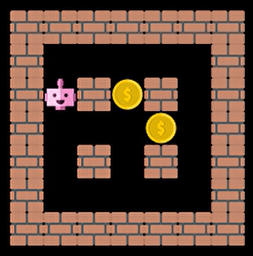
\includegraphics{images/coin_blocked.png}
	\caption{In this extract of Bomberman the agent is positioned only two tiles away from the closest coin, but a wall is blocking the direct way to the coin. So by moving up or down one tile the agent would be three tiles away from that coin. However, this step is necessary to get to the coin at all, so here it is not penalised to move away from the coin, like it normally is.}
	\label{fig:coin-blocked}
\end{figure}

\textbf{Rewarding each crate that will be destroyed by a dropped bomb and considering the necessity of a dropped bomb:}

Next we included two reward functions that are closely related to each other, namely a function counting and rewarding all crates that will be destroyed by a bomb dropped by our agent and another function penalising or rewarding the necessity of a bomb dropped by our agent. To count all crates that are lying in the bomb's explosion radius we have to check each tile that is impacted by the bomb for the existence of a crate. To do that we need to be sure that the index of the potential explosion radius is part of the game's field and if there is a crate it could be protected by a wall blocking the explosion. Every crate that will be destroyed by a bomb gives an extra 5 point reward. If no crate will be destroyed the reward is -5. 

Additionally, the bomb necessity reward function monitors if there is a opponent in a 7 $\times$ 7 field around the dropped bomb because this opponent could potentially move into the explosion radius. Every opponent fulfilling this condition brings an extra 2 point reward, while the action of dropping a bomb in a position where no opponent is in the 7 $\times$ 7 field and no crate will be destroyed results in a negative reward of 22.
\\ \\
\textbf{Punishment for a dropped bomb without an escape route:}

In regards to bombs dropped by our agent we introduced one more reward, as one of the worst moves an agent can do in this game is dropping a bomb that the agent cannot escape from. Consequently, we penalised this very hard with -100. To control if there is an escape route we initialized four variables, each variable illustrating one direction in which the agent could escape, with False. Then the implementation works its way from the outside to the inside, first looking if the tiles outside of the bomb's explosion radius in all four directions are free, which turns the boolean variable accordingly to True. Next, one tile closer to the bomb, we check if this tile is free and one of the adjacent tiles that are not affected by the explosion are free too. This would result in changing the corresponding direction variable to True as the agent would be able to escape to these adjacent tiles in time before the bomb goes off. However, if the tile on the way to the adjacent safety spots is blocked by a wall or crate the variable is changed back to False even when it could have been True before. This is done again for a tile even closer to the bomb, and so on, for all four directions. Concluding we have four variables that state whether in a direction, so to the bottom, top, left or right, there is an escape route or not. If any of these variable's values is True there is an escape route and the agent is rewarded with 2 for dropping a bomb that it can escape from. Otherwise, as mentioned before, the punishment is -100.
\\ \\
\textbf{Assess movements made by the agent in regards to all bombs on the field:}

Lastly, the agent has to pay attention to every bomb, not only its own bombs and eventually move to safety. With our final reward function called bomb radius we gave the agent positive feedback when moving away from a bomb and finding a safe spot and negative feedback if the agent moves back into a bomb radius or gets closer to a bomb. To do so, we first examine if the agent is positioned on the same spot as a bomb, so probably the bomb we are dealing with is a self dropped bomb. Then we use the function explained above that determines the possible directions that the agent can escape to and reward the agent for moving in a direction where it is possible to escape. On the other hand of course the agent is punished with a negative reward for going in a direction without a possibility to escape. 

If the agent is not positioned on the exact same x- and y-positions of a bomb but rather one coordinate, so either x- or y-coordinate, overlap with a bomb we have to take a couple of cases into consideration. First, is a wall protecting the agent from the explosion anyway? If the answer to this question is yes we are not interested in rewarding the move the agent does because it was not in danger in the first place, and cannot move into the danger zone of this bomb with one action. Without a protecting wall, the question is whether the agent is too close to a bomb, so that the explosion would kill the agent. In this case the agent gets a small reward for moving away but still being in the bomb's radius and a higher reward for moving to a tile that will not be affected by the bomb's explosion. However, if the agent does not move away it is punished. There is also the possibility that the agent was not in the bomb radius and moved into it, which gets punished as well. The same is done in the third case, that the agent had no overlapping coordinates but moved into the bombs radius.

The reward, no matter if positive or negative, determined by all the above mentioned if-cases is multiplied by 4 subtracted by the count down until the bomb explodes, which ranges from 3 to 0. So if the bomb was just dropped and has a count down number of 3, the reward stays the same as it is multiplied by 1.On the other hand, if the bomb goes off soon, so the count down number is 0 the reward is multiplied by 4. By including this multiplication we hoped to emphasize the need to get out of the way of a bomb if it detonates soon. Additionally, the agent should not hesitate to move through a bomb radius to, for example, come closer to a coin if the count down of a bomb is still high.
\\ 

All of these auxiliary rewards needed to be adjusted such that the agent understands the priorities of the game and does not make unnecessary moves due to bad rewarding. Eventually, our final agent learned how to play the game fairly efficient after a total of 100,000 rounds of training in different scenarios with different settings, which would not have been possible with only the standard rewards.

\newpage
\fancyhead[R]{Berkay Günes}
\subsubsection{Input features} \label{InFeatures}
It is important to preprocess the input to the Neural Network, else it would be difficult for the Network to determine the important parts out of the big feature state that is provided by the game environment.\\
We decided to limit the vision of the agent to a surrounding of a 7x7 grid. This gives the benefit of being able to train the agent on different game sizes and being able to scale the game without the agent losing information.\\ \\
Since Neural networks prefer working with ones and zeros we tried to separate each information as much as possible and not cramp all available informations into one array with different numbers.\\
Therefore we created three 7x7 arrays, that contain -1 for one type of information on that field and 1 for another. So one array has -1 for walls and 1 for crates, the second array has -1 for explosions and 1 for coins and the third array contains -1 for bombs and their range and 1 for opponents.\\
To give the agent a chance to have a sense for whats outside of his narrow world view, we implemented a 4x4 array that contains informations, whether there is a coin, crate, explosion/bomb or opponent to the right, left, top or bottom of the agent.\\ \\
So the input to our neural network contains three 7x7 arrays with a vision of its surroundings and a 4x4 array with an outside view.

% ----------------------------------------------------------------------------------------------------------------------------------------------

\subsubsection{Network structure} \label{NetworkS}

A significant part to how well the agent performs and its dependencies to learn are defined by its Neural Network structure.\\
We tried different approaches to determine what gives the agent the best possibility to master the game.\\
Our final agent has a Network that takes in four tensors and has an individual pipeline for each of these tensors in the first two layers. Afterwards they get connected into one fully connected layer before they connect to the output layer.\\
As described in \ref{InFeatures} we give our network three arrays with a 7x7 view around the agent. These array go each through a convolutional layer and get each passed into their own linear layer before they all get connected in the layer before the output.\\ \\
The idea behind this network structure is to let the network first process all informations on crates, walls, coins, bombs, explosions and opponents independently, before everything gets mushed together.

\newpage
\fancyhead[R]{Kevin Klein}
\subsection{second best agent}

In this section, we describe how we trained our second-best agent. This agent initially imitates 
the rule-based agent and then seeks further improvement through deep Q-learning.

\begin{figure}[H]
    \centering
    
    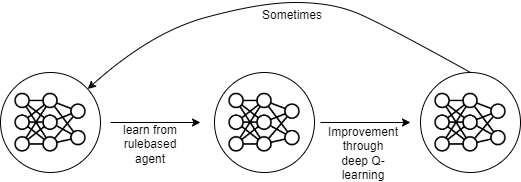
\includegraphics[width=\oneImgWidth]{images/training-strategy}%
    
    \captionadjust%
    \caption{\label{fig:training-strategy} Here is how we trained our second best model.
    }%
\end{figure}

Our initial idea was to develop an agent that starts by performing at the same level as the rule-based agent and then improves 
further through deep Q-learning. For this purpose, we had devised the following concept see \autoref{fig:training-strategy}.

Initially, our agent attempted to imitate the rule-based agent, as mentioned earlier. This was achieved through a classification approach. 
We collected the actions of the rule-based agent for each game state, and these actions served as the labels for the respective states. 
We gathered between 500,000 and 1,000,000 action-label pairs in this manner.
New data was added to the ReplayBuffer after each step until reaching the limit of 500,000 to 1,000,000 entries. 
After each round, specifically at the \verb|end_of_round| event, the following simplified function was executed to train our model.
Of course, the model was then also saved in an external file, which was achieved using Pickle.

\begin{lstlisting}[language=Python]
    ...
    
    def learn_rulebased_agent(model, labels, data, loss, opt, batch_size):
        train_ds = CTDataset(data, labels)
        train_dl = DataLoader(train_ds, batch_size=batch_size, shuffle=True)
        epoch_loss = 0

        ...

        for epoch in range(NUM_EPOCH):
            print("epoch %d / %d" % (epoch + 1, NUM_EPOCH))
            for i, (x, y) in enumerate(train_dl):
                opt.zero_grad()
                pred = model(x)
                loss_value = loss(pred, y) 
                loss_value.backward() 
                opt.step()
                epoch_loss += loss_value.item() 

            if epoch_loss <= 1e-5:
                break

            print(f"loss/epoch: {epoch_loss}")
            epoch_loss = 0      

    ...
    
\end{lstlisting}

First, we pass the model to the function that we want to train, followed by the labels, 
which represent the actions of the rule-based agent, and the data, which corresponds to the states. 
Then, we provide the loss function and optimizer, and finally, the batch size. We found that a batch size of 1024 worked well for us, 
especially as the model had more data to train on when the ReplayBuffer became fuller. We did experiment with other batch sizes,
but if the batch size was too small, it took a long time for the loss function to converge to 0 (which it didn't entirely reach).

We achieved good results when the \verb|num_epoch| was initially set at 2000, which we later increased to 5000 during training. 
Additionally, we sometimes had to remove older data from the ReplayBuffer to ensure that the model continuously learned from new games. 
It was also worthwhile to reduce the view box to 7x7 because it significantly reduced the number of possible states. 
After 4-5 days of training, our model became reasonably proficient at playing the game. While it couldn't perfectly mimic the rule-based agent, 
as the agent occasionally had to make random moves when there were no more items in its 7x7 view box, we still found the results quite satisfactory.

Afterward, we attempted to enhance the model using Q-learning. For this, we utilized the reward function from our best agent in the first project. 
Unfortunately, this approach didn't work well; the agent's performance deteriorated, and eventually, it struggled to play the game effectively. 
We saw improvement when we alternated training the model with the rule-based agent and then applied deep Q-learning see \autoref{fig:training-strategy}. 
However, even in this scenario, 
the results were significantly worse compared to when our model was solely imitating the rule-based agent.

In the end, we were unable to improve the agent using Q-learning beyond the level of our initial project, 
which we naturally submitted. We also considered reasons why we couldn't enhance the agent pre-trained with rule-based 
data using deep Q-learning. The main issue likely stems from optimizing the model with vastly different values when it imitates 
the rule-based agent compared to when it undergoes deep Q-learning. In the first case, the model is optimized with one-hot encoded 
actions of the rule-based agent, while in the latter case, it's optimized with the values of the reward function and the next states.